%%%%%%%%%%%%%%%%%%%%%%%%%%%%%%%%%%%%%%%%%%%%%%%%%%%%%%%%%%%%%%%%%%%%%%%%%%%%%%%%%%%%%%%%%%%%%%%%%%%
\chapter{Conclusões e trabalho futuro}


\section{Conclusões}



O objetivo deste trabalho consistiu em desenhar e desenvolver um sistema de informação que permitisse o armazenamento dos dados provenientes de um sistema de sensores para monitorizar e controlar o cultivo da Salicórnia. O trabalho prático desta dissertação foi elaborado tendo por base este objetivo geral e pode-se afirmar que este foi cumprido com sucesso. Este sistema disponibiliza uma plataforma \textit{web} que permite aos utilizadores consultar os dados obtidos pelos sensores e atuar remotamente permitindo melhorar as condições de cultivo. Para além disso, foi disponibilizada uma \ac{API} que permite o acesso a serviços do sistema, possibilitando a criação de novas aplicações. Para simular e testar o cenário pretendido, foi criado um protótipo de \textit{hardware}. Adicionalmente, foi criado um sistema de videovigilância para incorporar nas quintas onde se faz a produção desta planta. Todas estas funcionalidades vão de encontro aos objetivos específicos apresentados na secção \ref{objectivos}, à exceção da incorporação do sistema de videovigilância com o algoritmo de deteção de intrusos. Contudo, este algoritmo foi apresentado e testado para alguns cenários, permitindo concluir que os parâmetros utilizados dependem do ângulo e da posição da câmara.  Na figura \ref{resumo} encontra-se um esquema que permite resumir todo o trabalho realizado nesta dissertação. 

\begin{figure}[h]
	\centering
	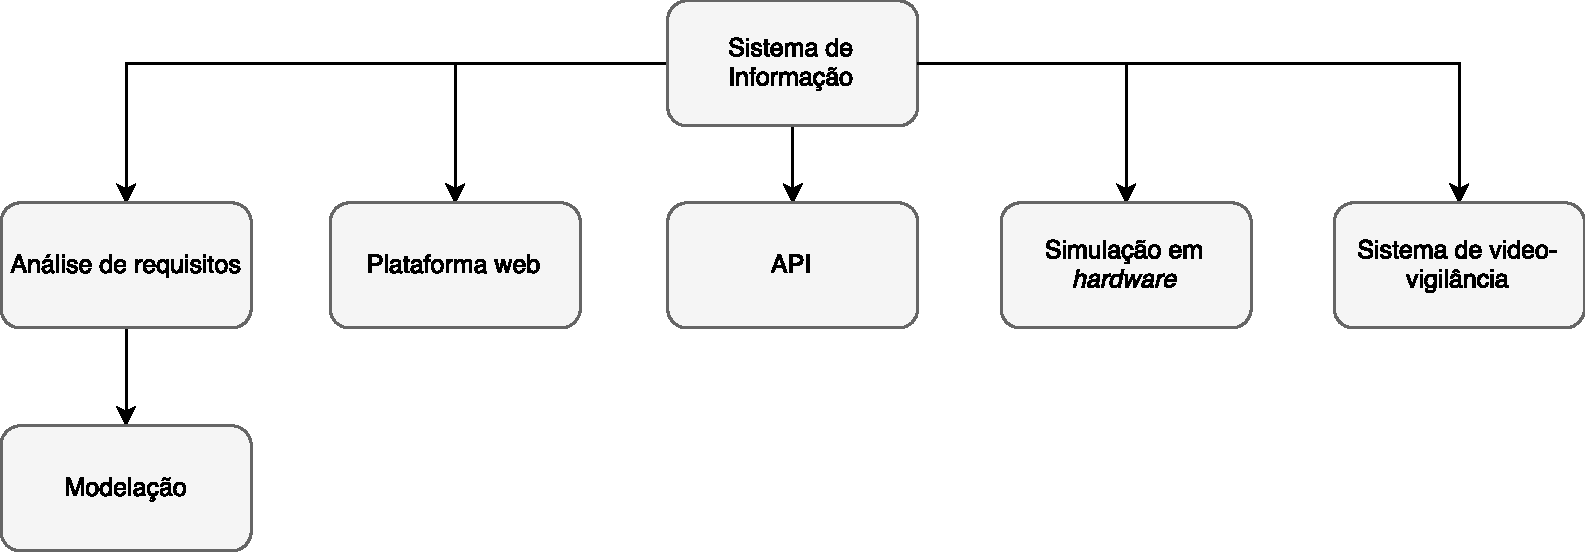
\includegraphics[width=0.68\linewidth]{esquemas/conclusaofinal.pdf}
	\caption{Esquema resumo do trabalho desenvolvido}
	\label{resumo}
\end{figure}



Toda a modelação do sistema vai de encontro aos requisitos inicialmente especificados pelo cliente, bem como aos definidos durante o desenvolvimento deste trabalho. Desta forma, é permitido que o sistema seja genérico e passível de ser aplicado em qualquer cenário, seguindo a arquitetura definida. Adicionalmente aos objetivos desta dissertação, planeou-se a arquitetura e criou-se um \textit{mockup} de uma aplicação \textit{mobile}, estando esta prevista pelos requisitos do cliente. Embora esta aplicação tenha sida sugerida pelo cliente não houve tempo de a concretizar. 


O sistema de informação criado poderá ser utilizado como ponto de partida para qualquer objetivo, desde que respeite a arquitetura inicialmente definida, isto é, composta por \textit{Controller Modules} e \textit{Sensor Modules}. 



\section{Problemas encontrados}


Durante o desenvolvimento e implementação deste sistema surgiram alguns problemas, tanto pontuais e de correção simples, como
problemas estruturais, que levaram a algumas mudanças. Alguns dos problemas estruturais estão relacionados com o modelo de dados, em que foram adicionados novos campos às tabelas existentes, quer para o suporte de novas funcionalidades, quer para aumentar o comportamento dinâmico do sistema.


Tal como referido anteriormente, não foi possível incorporar o sistema de videovigilância com o algoritmo de deteção de intrusos. Para tal, pretendia-se utilizar a \ac{API} do Youtube. Esta utilização não foi possível devido à reduzida documentação da \ac{API} que dificultou a sua implementação. Para além disso, existem poucos exemplos que permitem entender eficazmente a utilização da referida \ac{API}. 

Um outro obstáculo na realização deste trabalho, foi o facto de o projeto não ser financiado por parte do cliente, impossibilitando assim, a compra de um sensor de salinidade (condutividade), sendo este um dos parâmetros mais importante de monitorizar no controlo do cultivo da Salicórnia. 




%projeto sem financiamento por nao foram utilizados sensores de salinidade: 


%justificar o falta fazer se é estável pode ser usado como porto de partida para 

%O que podia ser feito: testes de usabilidade, medir tempos de resposta do web site; \\



\section{Trabalho futuro}



Como trabalho futuro, propõe-se realizar alguns testes de usabilidade à aplicação \textit{web} permitindo verificar o grau de facilidade/dificuldade de utilização deste \textit{software}.  Como mencionado anteriormente, o cliente do sistema pretende que exista um aplicação móvel que possibilite monitorizar o seu cultivo, sendo esta considerada como trabalho futuro. Outra situação que considerei diferenciadora prende-se com automatizar o registo dos módulos através da leitura de um código \ac{QR} podendo este mecanismo ser incorporado na aplicação \textit{mobile}. Relativamente ao sistema de videovigilância, tenciona-se testar o algoritmo apresentado numa câmara térmica (infravermelho) permitindo a deteção de intrusos durante a noite. Por fim, pretende-se criar um circuito impresso do protótipo de \textit{hardware} desenvolvido. 











 
